%==============================================================================
% Sjabloon onderzoeksvoorstel bachproef
%==============================================================================
% Gebaseerd op document class `hogent-article'
% zie <https://github.com/HoGentTIN/latex-hogent-article>

% Voor een voorstel in het Engels: voeg de documentclass-optie [english] toe.
% Let op: kan enkel na toestemming van de bachelorproefcoördinator!
\documentclass{hogent-article}

\usepackage{graphicx}
\graphicspath{{./img/}}

% Invoegen bibliografiebestand
\usepackage[backend=biber,style=apa]{biblatex}
\DeclareLanguageMapping{dutch}{dutch-apa}
\addbibresource{references.bib}
\usepackage{hyperref}
% Informatie over de opleiding, het vak en soort opdracht
\studyprogramme{Professionele bachelor toegepaste informatica}
\course{Bachelorproef}
\assignmenttype{Onderzoeksvoorstel}
% Voor een voorstel in het Engels, haal de volgende 3 regels uit commentaar
% \studyprogramme{Bachelor of applied information technology}
% \course{Bachelor thesis}
% \assignmenttype{Research proposal}

\academicyear{2023-2024} 

% TODO: Werktitel
\title{Vergelijkende studie van Augmented Reality ondersteunde mobiliteitstool voor personen met een mentale beperking: een proof of concept benadering.}

% TODO: Studentnaam en emailadres invullen
\author{Robin De Waegeneer}
\email{robin.dewaegeneer@student.hogent.be}

% TODO: Geef de co-promotor op
\supervisor[Co-promotor]{T. Aelbrecht (HoGent, \href{mailto:thomas.aelbrecht@hogent.be}{thomas.aelbrecht@hogent.be})}

% Binnen welke specialisatierichting uit 3TI situeert dit onderzoek zich?
% Kies uit deze lijst:
%
% - Mobile \& Enterprise development
% - AI \& Data Engineering
% - Functional \& Business Analysis
% - System \& Network Administrator
% - Mainframe Expert
% - Als het onderzoek niet past binnen een van deze domeinen specifieer je deze
%   zelf
%
\specialisation{AI \& Data Engineering}
\keywords{Mobiliteitstool, mentale beperking, AR}

\begin{document}

  \begin{abstract}
    Dit onderzoek richt zich op de integratie van AR voor de optimalisatie van interactieve mobiliteitstools voor mensen met een mentale beperking. Mobiliteit is een belangrijk aspect van het dagelijkse leven en vormt een specifieke uitdaging voor mensen met een verstandelijke beperking. Startpunt van het onderzoek zijn reeds bestaande tools die aan de hand van augmented reality (AR) tot een volledig POC zullen uitgewerkt worden. Dankzij een bevraging van de stakeholders wil het onderzoek bijkomende inzichten creëren zowel omtrent de doelgroep als de concrete oplossingen. Binnen de uitwerking van de POC is gepland om een groep kinderen met de ontworpen app te laten experimenteren om na te gaan hoe ze zich beter kunnen verplaatsen met de AR ondersteunde applicaties. Uit de vergelijkende studie wordt verwacht dat specifieke AR functionaliteiten zullen worden geïdentificeerd voor de doelgroep. Bovendien zal dankzij een testfase van de POC het effectieve gebruiksgemak worden beoordeeld. Als conclusie zal deze studie een duidelijk lastenboek afleveren voor verdere ontwikkeling van een aangepaste mobiliteitstool voor mensen met een mentale beperking.
  \end{abstract}

\tableofcontents

\bigskip

\section{Inleiding}%
    \label{sec:inleiding}
    
    Mensen met een mentale beperking ondervinden bij het gebruik van bestaande mobiliteitstools problemen, omdat deze uitgaan van een basisniveau lees- en schrijfvaardigheid waarover zij niet beschikken. Bovendien is in sommige gevallen ook hun tijds- en ruimtebesef gelimiteerd. Het globale objectief van het onderzoek is een tool te ontwikkelen om deze mensen via  Augmented Reality (AR) ondersteuning deze op een efficiënte en veilige manier te gebruiken. De POC wordt zo eenvoudig mogelijk ontwikkeld, zodat ze gestructureerd hun weg kunnen vinden met behulp van het openbaar vervoer. Door bestaande tools te screenen, al dan niet gericht op onze doelgroep, en deze af te toetsen door bevraging van verschillende stakeholders, wordt een meer optimale tool in kaart gebracht. Kort gezegd: hoe geraakt iemand die niet kan (klok)lezen zonder enige begeleiding van punt A naar punt B met visuele en/of auditieve signalen aan de hand van AR binnen het juiste tijdsbestek.
    We zijn ervan overtuigd dat deze mobiliteitstool een grote impact en meerwaarde zal hebben voor deze doelgroep door hun limieten te verleggen en zelfstandigheid te vergroten.
    
    \section{Literatuurstudie}%
    \label{sec:literatuurstudie}
    
    % Refereren naar de literatuur kan met:
    % \autocite{BIBTEXKEY} -> (Auteur, jaartal)
    % \textcite{BIBTEXKEY} -> Auteur (jaartal)
    De literatuurstudie zal een overzicht maken van de bestaande tools zoals de applicaties van NMBS, De Lijn en standaard routeplanners. Deze applicaties en websites zijn gebaseerd op het principe dat de gebruiker zelfstandig een adres en tijdstip zelf kan ingeven en maken niet altijd gebruik van locatiebepaling, wat voor de doelgroep een duidelijke hinderpaal is.
    
    Daarnaast zullen diverse AR methodes binnen de huidige state of the art vergeleken worden voor het verbeteren van de gebruikerservaring. Mapbox AR maakt gebruik van points of interest terwijl Google Maps AR inzet op multidimensionele visualisatie om de gebruiker comfortabel aan te sturen tijdens het navigeren. Met behulp van de camera van het mobiele apparaat worden real-time beelden van de omgeving vastgelegd, waarbij digitale routeaanwijzingen over de werkelijke beelden worden geprojecteerd. Dit zorgt voor een intuïtieve en praktische navigatie-ervaring, vooral in stedelijke gebieden waar traditionele kaarten mogelijk minder effectief zijn. 
    
    Mapbox AR onderscheidt zich door zijn typische karakteristiek van geavanceerde aanpasbaarheid en integratiemogelijkheden. Deze tool biedt ontwikkelaars een krachtig platform waarmee ze op maat gemaakte augmented reality-toepassingen kunnen creëren, variërend van navigatie tot locatiegebaseerde informatie. Hierdoor hebben ontwikkelaars de flexibiliteit om kaartgegevens aan te passen, aangepaste overlays toe te voegen en de gebruikerservaring te optimaliseren voor specifieke doeleinden. Beide tools vertegenwoordigen technologieën binnen het domein van augmented reality en kaartnavigatie. Ze tonen de evolutie aan van traditionele kaartapplicaties naar meer dynamische, op AR gebaseerde oplossingen.  
     
    Ook Koombea verhoogt de gebruikerservaring en met AR City komt de locatie effectief tot leven dankzij bijkomende informatie. Sygic werd specifiek ontwikkeld voor auto GPS-systemen om de bestuurderservaring te optimaliseren, maar kan een toegevoegde waarde hebben wanneer de gebruiker tijdens een busrit het traject mee wil opvolgen. Functionaliteiten van elk deze tools zullen gescreend worden om te bepalen of zij in aanmerking komen voor integratie in de POC. 
    
    De implementatie van locatiegevoelige informatie in combinatie met de AR visualisatie neemt diverse barrières weg voor de doelgroep. Zij hoeven immers niet het adres te kennen van hun startpunt. Het eindpunt kunnen ze bv. omschrijven via een pictogram zoals deze gebruikt worden in Sclera. Deze pictogrammen worden standaard aangeleerd bij onze doelgroep ter bevordering van hun communicatie en visualisatie van hun dagplanning.
    
    Naast het openbaar vervoer kunnen andere systemen zoals Dott en Villo worden overwogen omdat dergelijke fietsen en steps verspreid staan in diverse steden. Ze bieden een bijkomende optie voor het verplaatsen van punt A naar punt B op een efficiënte manier.
    
    Op hardwaregebied ontwikkelde Google in 2014 een smart device genaamd Google Glasses. Deze brillen hadden als doel om AR een extra boost te geven aan de hand van een concreet concept. Het product kreeg een tweede versie in 2017, als ondernemingseditie, maar had geen succes en eerder dit jaar in maart 2023 kondigde Google aan dat ze het project stopzetten \autocite{Gvora2023}.
   
    Tot slot geldt dat de doelgroep die niet in staat is te lezen of schrijven, wel gebruik kan maken van text-to-speech functionaliteit om de gewenste locatie te omschrijven. De tool moet met andere woorden ook deze stemherkenning als ondersteuning bieden. Dankzij artificiële intelligentie (AI) wordt dan de beste route berekent en tevens de beste manier om daar gemakkelijk te geraken\autocite{Soni2023a}. Het gebruik van datastructuren zal toelaten deze locatie informatie te linken aan het routepatroon\autocite{Ruta2010}. Bovendien kunnen deze patronen potentiële knelpunten identificeren, hulp bieden bij het optimaliseren van routes als er verkeerswerken of files zijn. De noodzaak van dit systeem zijn realtime gegevens waarbij samenwerking met belanghebbende belangrijk is \autocite{Ciravegna2018}. 
    
    Het opzetten van een meta model kan begeleiders van mensen met een matige mentale beperking helpen met het navigeren naar een juiste plaats. Door gegevensverzameling kan er aan de hand van algoritmes voorspellingen gemaakt worden wat voor deze persoon de favoriete manier van verplaatsen is of favoriete route is om te volgen naar het werk \autocite{Stepanov2003}. Als laatste kan er gebruik gemaakt worden van IoT (Internet of Things) tools voor het slim communiceren tussen verschillende apparatuur wat kan leiden tot nog betere prestaties in verplaatsing en routeberekening \autocite{Fatnassi2015}.
    

    
    \section{Methodologie}% \\
   
    De methodologie van het onderzoek bestaat uit een aantal belangrijke deelstappen waaronder literatuurstudie, een requirementsanalyse door middel van bevraging van de noden bij de stakeholders, definitie van de software inclusief AR opties, mogelijke hardwarecomponenten voor implementatie, uitwerking van de proof of concept, een praktijkexperiment in meerdere fasen, het formuleren van de conclusies en de scriptie. De hoofdvraag omvat diverse delenaspecten zoals kan locatiebepaling helpen om zelfstandige input van de gebruikers te omzeilen. Anderzijds zal ook het deelaspect van de specifieke communicatiemogelijkheden voor mensen met een beperking worden geëvalueerd. Tot slot brengt de integratie van AR een toegevoegde waarde omtrent veiligheidsgevoel en comfort, wat moet blijken uit de feedback van de praktijktesten.
    
    \textbf{Bevraging van de noden} \\
    
    Na de nodige research online en in bestaande applicaties van huidige aanbieders, is een bevraging van diverse stakeholders gepland. Aan de hand van interviews met De Lijn, NMBS, begeleidingsorganisaties en vakexperten die mensen met een matige mentale beperking begeleiden, worden inzichten verworven over de huidige mogelijkheden en de specifieke noden. Hiervoor zullen een aantal sleutelorganisaties benaderd worden zoals het VAPH (Vlaams Agentschap voor Personen met een Handicap), Tanderuis (gespecialiseerd in autismespectrumstoornis) en Fiola (begeleiding mensen met mentale beperking).

    Welke zijn de basisvoorwaarden voor een toegankelijke applicatie en welke aangepaste communicatiemiddelen kunnen praktisch ingezet worden. Deze bevraging zal het lastenboek definiëren voor onze proof of concept en mogelijkheden voor samenwerking verduidelijken. 
    
    \textbf{Onderzoek Software} \\
    
    Op basis van de bevragingen uit bovenstaande fase start de ontwikkeling van de softwaremogelijkheden. Met hogervermelde uitkomsten zal een gedetailleerde beschrijving opgemaakt worden. Hierin zullen 3 grote rubrieken aan bod komen:
    
    \begin{enumerate}
        \item \textbf{Functies}: Een lijst van alle nodige functies in de app (location tracking, text-to-speech, voorleesfunctie, language models, visualisatietypes, Sclera pictogrammen)
        \item \textbf{Integraties}: Een omschrijving van mogelijke AR integraties (Google Maps, Mapbox, Koombea, AR City, Sygic)
        \item \textbf{Werkwijze en denkpatronen}:Een selectie van enkele mogelijke manieren waarmee interactie kan geïnitieerd worden inclusief AR (kleuren, geluiden, patronen, figuren, ...)
    \end{enumerate}

    Uiteindelijk zal een compilatie gemaakt worden van de beste opties en combinaties om verder uit te werken in de proof of concept.
    
    \textbf{Hardwarecomponenten} \\
    
    Hierbij wordt afgetoetst welke mogelijkheden voor handen zijn om de software in werking te laten treden. Om te achterhalen wat de beste optie(s) zijn, zullen de inzichten, verworven in de ontwikkeling van het softwaregedeelte, geïmplementeerd worden via verschillende platformen zoals een tablet, een smartwatch, een smartphone of een combinatie ervan.
    
    \section{Proof-of-concept}% \\
    \label{sec:proof-of-concept}
    De POC zal worden uitgewerkt op een smartphone voor een aantal specifieke routes waarin minstens 1 openbaar vervoersmiddel (trein, bus) is geïntegreerd.
    
    \section{Praktijkexperiment}
    \label{sec:praktijkexperiment}
    Een geselecteerde doelgroep zal de smartphone met applicatie uittesten in twee fasen en nadien feedback geven over het gebruiksgemak. In test 1 worden de locaties A en B vooraf bepaald en ingevuld door een begeleider. Na afloop geven de gebruikers feedback over de interactieve ervaring gecreëerd dankzij AR. In de tweede test zullen de gebruikers zelf via een omschrijving het eindpunt invullen. Hun startpunt wordt bepaald op basis van de locatiegegevens. Een van de hoger vermelde begeleidingsorganisaties kan hierbij helpen en tevens feedback geven over het experiment en de integratie van de specifieke communicatiemiddelen zoals Sclera.



    \section{Verwachte resultaten}% \\
    \label{sec:verwachte-resultaten}
    
    Uit de screening van bestaande tools zullen nuttige functies worden gebruikt als bouwstenen voor de POC van dit onderzoek. Dankzij de inzichten verworven in de bevraging van de noden en gesprekken met diverse stakeholders zal deze POC zo functioneel mogelijk zijn voor de specifieke doelgroep. Tot slot zal dankzij een experimentele fase nagegaan worden hoe efficiënt de concrete uitwerking is en welke positieve impact AR implementatie kan hebben.
    
    
    \section{Discussie, conclusie}%
    \label{sec:discussie-conclusie}
    In essentie kan worden gesteld dat er al enkele bruikbare tools ontwikkeld zijn, maar deze niet (volledig) aan de noden voldoen voor mensen met een matige mentale beperking. Deze hulpmiddelen vereisen nog steeds een redelijke kennis in het gebruik. Daarom wordt, na bevragingen, een POC opgesteld aan de hand van verworven inzichten. De bekomen resultaten van de literatuurstudie, in combinatie met de bevragingen en gebouwde POC, zullen een duidelijk beeld schetsen voor de samenwerking met een hardwarebedrijf of AR bedrijf. Als resultaat hierop wordt meteen ook nagedacht over extra functies en integraties die dan samengevat worden als opsomming met latere innovaties.

    % \section{Verloop}%
    % \label{sec:verloop}
    % In de flowchart wordt een beeld geschetst van de logische stappen waaruit het onderzoek bestaat. De tijdslijn van de opeenvolgende fasen is uitgezet in een Gantt-chart. De bevraging van de stakeholders wordt opgestart zodra een eerste beeld is gevormd via screening van bestaande tools. De software uitwerking van de POC start zodra al deze resultaten verwerkt zijn tot een duidelijke omschrijving van de noden en functionaliteiten. Met de eerste POC resultaten kunnen in parallel ook hardwarecomponenten gezocht worden. Bij het afronden van deze concrete uitwerkingsfasen wordt verder aangevuld met mogelijke latere innovaties. De resultaten omvatten duidelijke keuzes voor de finale POC en in de conclusies worden deze opnieuw getoetst aan de initiële doelstellingen en verwachtingen. Het neerschrijven van alle bevindingen in de scriptie loopt gedurende het volledige traject van het onderzoek. \\\\
    
    \textbf{Flowchart} \\\\
    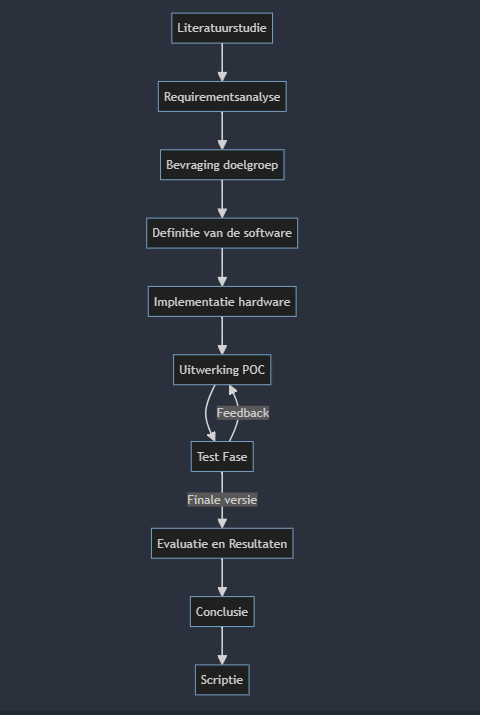
\includegraphics[width=\columnwidth,height=11cm]{flow}
    
    % \vspace{5mm}
    
    % \textbf{Gantt-chart} \\\\
    % 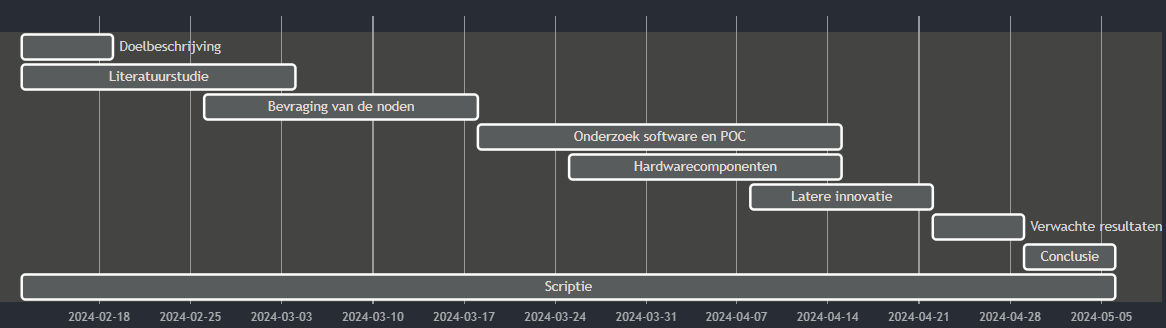
\includegraphics[width=\columnwidth]{gantt}
    % %---------- Inleiding ---------------------------------------------------------

\section{Introductie}%
\label{sec:introductie}

    personen met een mentale beperking ondervinden bij het gebruik van bestaande mobiliteits\-tools problemen, omdat deze uitgaan van een basisniveau lees- en schrijfvaardigheid waarover zij dikwijls niet beschikken. 
    Bovendien is in sommige gevallen ook hun tijds- en ruimtebesef gelimiteerd. 
    Het globale objectief van het onderzoek is een tool te ontwikkelen om deze doelgroep via Augmented Reality (AR) ondersteuning te bieden om bestaande mobiliteitstools op een efficiënte en veilige manier te gebruiken.
    De Proof-of-Concept (POC) wordt zo eenvoudig mogelijk ontwikkeld, zodat ze gestructureerd hun weg kunnen vinden met behulp van het openbaar vervoer. 
    Door bestaande tools te screenen, al dan niet gericht op onze doelgroep, en deze af te toetsen door bevraging van verschillende stakeholders, wordt een meer optimale tool in kaart gebracht. 
    Kort gezegd: hoe geraakt iemand die niet kan (klok)lezen zonder enige begeleiding van punt A naar punt B met visuele en/of auditieve signalen aan de hand van AR binnen het juiste tijdsbestek? We zijn ervan overtuigd dat deze mobiliteitstool een grote impact en meerwaarde zal hebben voor deze doelgroep door hun grenzen te verleggen en zelfstandigheid te vergroten. De hoofdvraag kan hiertoe in enkele deelvragen onderverdeeld worden;
    
    \begin{enumerate}
        \item Welke problemen ervaren personen met een mentale beperking bij het gebruik van bestaande mobiliteitstools?
        \item Hoe kan Augmented Reality (AR) ge-\\integreerd worden in bestaande mobiliteits\-tools?
        \item Hoe kunnen AR en locatiebepaling worden ingezet om personen met een mentale beperking te ondersteunen bij het navigeren met het openbaar vervoer?
        \item Op welke manieren kan de mobiliteitstool worden aangepast aan de specifieke behoeften en voorkeuren van de doelgroep?
        \item Hoe kan een praktijkexperiment worden opgezet om de efficiëntie en gebruiksvriendelijkheid van de ontwikkelde mobiliteitstool te evalueren bij de doelgroep?
        \item Welke visuele en/of auditieve signalen zijn het \\meest efficiënt?
    \end{enumerate}

%---------- Stand van zaken ---------------------------------------------------

\section{State-of-the-art}%
\label{sec:state-of-the-art}
  
  De literatuurstudie zal zich richten op het verkennen van de mobiliteitsbehoeften van de doelgroep en het bespreken van bestaande tools en technologieën die hen kunnen ondersteunen bij het navigeren en reizen.
  Mensen met een beperking worden vaak geconfronteerd met uitdagingen bij het plannen en uitvoeren van verplaatsingen. Afhankelijk van hun type beperking kunnen deze noden bovendien sterk variëren. Bij autismespectrumstoornis (ASS) werden diverse aspecten omtrent tijdsbesef samengevat door Prof. Degrieck \autocite{Degrieck2014}.
  Een grote gemeenschappelijke deler bij deze doelgroep is de nood aan eenduidige structuur, vaak visueel ondersteund en de afwezigheid van onnodige prikkels. De website van Participate\footnote{\url{https://nl.participate-autisme.be}} bundelt hieromtrent heel wat ervaringsgerichte informatie via hun FAQ en enkele blogs. Zeker in de context van ASS is een advertentie-luwe omgeving met enkel essentiële informatie een absolute noodzaak \autocite{Roeyers2014}. 
  De mogelijkheid om te kiezen voor een klassiek klokbeeld in plaats van het digitale beeld of een keuze voor bepaalde lettertypes kan voor mensen met een laag IQ die slechts bepaalde letter- en cijfercombinaties kunnen memoriseren het verschil maken \autocite{Uyttersprot2021,Tytgat2014,DeGraaf2001}. Welke technologieën dragen het beste bij tot begrijpbaarheid en kunnen zo hun mobiliteit en zelfstandigheid verbeteren?
  Een aantal belangrijke aandachtspunten en best practices voor mensen met een beperking zullen vanuit deze invalshoeken worden onderzocht, zoals de noodzaak van locatiegebaseerde informatie, de mogelijkheid van het gebruik van pictogrammen voor het beschrijven van locaties, en de integratie van spraakherkenning voor gebruikers die niet kunnen lezen of schrijven.Daarnaast zullen verschillende soorten mobiliteitsapps worden besproken, waaronder applicaties van openbare vervoersmaatschappijen zoals NMBS\footnote{\url{https://www.belgiantrain.be/nl}} en De Lijn\footnote{\url{https://www.delijn.be/nl/}}, standaard routeplanners en andere specifieke mobiliteitsapps zoals Dott\footnote{\url{https://ridedott.com/nl/}} en Villo\footnote{\url{https://www.villo.be/nl/home}} voor fietsen en steps. Het doel is om te analyseren hoe deze apps momenteel functioneren en welke verbeteringen nodig zijn om ze toegankelijker te maken voor mensen met een beperking.
  Deze applicaties en websites zijn gebaseerd op het principe dat de gebruiker zelfstandig een adres en tijdstip zelf kan ingeven en maken niet altijd gebruik van locatiebepaling, wat voor de doelgroep een duidelijke hinderpaal is.
  Daarnaast zullen diverse Augmented Reality (AR) methodes binnen de huidige state of the art vergeleken worden voor het verbeteren van de gebruikerservaring.
  Mapbox AR\footnote{\url{https://www.mapbox.com/augmented-reality}} maakt gebruik van points of interest terwijl Google Maps AR \footnote{\url{https://arvr.google.com}} inzet op multidimensionele visualisatie om de gebruiker comfortabel aan te sturen tijdens het navigeren.
  Met behulp van de camera van het mobiele apparaat worden real-time beelden van de omgeving vastgelegd, waarbij digitale routeaanwijzingen over de werkelijke beelden worden geprojecteerd.
  Dit zorgt voor een intuïtieve en praktische navigatie-ervaring, vooral in stedelijke gebieden waar traditionele kaarten mogelijk minder effectief zijn.
  Mapbox AR onderscheidt zich door zijn typische karakteristiek van geavanceerde aanpasbaarheid en integratiemogelijkheden.
  Deze tool biedt ontwikkelaars een krachtig platform waarmee ze op maat gemaakte augmented reality-toepassingen kunnen creëren, variërend van navigatie tot locatiegebaseerde informatie.
  Hierdoor hebben ontwikkelaars de flexibiliteit om kaartgegevens aan te passen, aangepaste overlays toe te voegen en de gebruikerservaring te optimaliseren voor specifieke doeleinden.
  Beide tools vertegenwoordigen technologieën binnen het domein van augmented reality en kaartnavigatie. Ze tonen de evolutie aan van traditionele kaartapplicaties naar meer dynamische, op AR gebaseerde oplossingen.
  Ook Koombea\footnote{\url{https://www.koombea.com}} verhoogt de gebruikerservaring en met AR City\footnote{\url{https://arcitygame.nl}} komt de locatie effectief tot leven dankzij bijkomende informatie.
  Sygic\footnote{\url{https://www.sygic.com}} werd specifiek ontwikkeld voor auto GPS-systemen om de bestuurderservaring te optimaliseren, maar kan een toegevoegde waarde hebben wanneer de gebruiker tijdens een busrit het traject mee wil opvolgen.
  De implementatie van locatiegevoelige informatie in combinatie met de AR visualisatie neemt diverse barrières weg voor de doelgroep.
  Zij hoeven immers niet het adres te kennen van hun startpunt. Het eindpunt kunnen ze bv. omschrijven via een pictogram zoals deze gebruikt worden in Sclera\footnote{\url{https://www.sclera.be/nl/picto/overview}}.
  Deze pictogrammen worden standaard aangeleerd bij onze doelgroep ter bevordering van hun communicatie en visualisatie van hun dagplanning.
  Naast het openbaar vervoer kunnen andere systemen zoals Dott en Villo worden overwogen omdat dergelijke fietsen en steps verspreid staan in diverse steden.
  Ze bieden een bijkomende optie voor het verplaatsen van punt A naar punt B op een efficiënte manier.
  Op hardwaregebied ontwikkelde Google in 2014 een smart device genaamd Google Glasses.
  Deze brillen hadden als doel om AR een extra boost te geven aan de hand van een concreet concept.
  Het product kreeg een tweede versie in 2017, als ondernemingseditie, maar had geen succes en eerder dit jaar in maart 2023 kondigde Google aan dat ze het project stopzetten \autocite{Gvora2023}.
  Tot slot geldt dat de doelgroep die niet in staat is te lezen of schrijven, wel gebruik kan maken van text-to-speech functionaliteit om de gewenste locatie te omschrijven.
  De tool moet met andere woorden ook deze stemherkenning als ondersteuning bieden.
  Dankzij artificiële intelligentie (AI) wordt dan de relatief beste route berekent en tevens de beste manier om daar eenvoudig te geraken \autocite{Soni2023a}.
  Het gebruik van datastructuren zal toelaten deze locatie informatie te linken aan het routepatroon \autocite{Ruta2010}.
  Bovendien kunnen deze patronen potentiële knelpunten identificeren, hulp bieden bij het optimaliseren van routes als er verkeerswerken of files zijn.
  De noodzaak van dit systeem zijn realtime gegevens waarbij samenwerking met belanghebbende belangrijk is \autocite{Ciravegna2018}.
  Het opzetten van een meta model kan begeleiders van mensen met een matige mentale beperking helpen met het navigeren naar een juiste plaats.
  Door gegevensverzameling kan er aan de hand van algoritmes voorspellingen gemaakt worden wat voor deze persoon de favoriete manier van verplaatsen is of favoriete route is om te volgen naar het werk \autocite{Stepanov2003}.
  Als laatste kan er gebruik gemaakt worden van Internet of Things (IoT) tools voor het slim communiceren tussen verschillende apparatuur wat kan leiden tot nog betere prestaties in verplaatsing en routeberekening \autocite{Fatnassi2015}.

% Voor literatuurverwijzingen zijn er twee belangrijke commando's:
% \autocite{KEY} => (Auteur, jaartal) Gebruik dit als de naam van de auteur
%   geen onderdeel is van de zin.
% \textcite{KEY} => Auteur (jaartal)  Gebruik dit als de auteursnaam wel een
%   functie heeft in de zin (bv. ``Uit onderzoek door Doll & Hill (1954) bleek
%   ...'')

%---------- Methodologie ------------------------------------------------------
\section{Methodologie}%
\label{sec:methodologie}

De methodologie van het onderzoek bestaat uit een aantal belangrijke deelstappen waaronder literatuurstudie, een requirementsanalyse door middel van bevraging van de noden bij de stakeholders, definitie van de software inclusief Augmented Reality (AR) opties, mogelijke hardwarecomponenten voor implementatie, uitwerking van de Proof-of-Concept (POC), een praktijkexperiment in meerdere fasen, het formuleren van de conclusies en de scriptie. De hoofdvraag omvat diverse deelaspecten zoals ``kan locatiebepaling helpen om zelfstandige input van de gebruikers te omzeilen''. Anderzijds zal ook het deelaspect van de specifieke communicatiemogelijkheden voor mensen met een beperking worden geëvalueerd. Tot slot brengt de integratie van AR een toegevoegde waarde omtrent veiligheidsgevoel en comfort, wat moet blijken uit de feedback van de praktijktesten. Na de nodige research online en in bestaande applicaties van huidige aanbieders, is een bevraging van diverse stakeholders gepland. Aan de hand van interviews met Fiola\footnote{\url{https://fiolavzw.be}} (begeleiding mensen met mentale beperking), Tanderuis\footnote{\url{https://www.tanderuis.be}} (gespecialiseerd in autismespectrumstoornis), begeleidingsorganisaties en vakexperten die mensen met een matige mentale beperking begeleiden, worden inzichten verworven over de huidige mogelijkheden en de specifieke noden. Welke zijn de basisvoorwaarden voor een toegankelijke applicatie en welke aangepaste communicatiemiddelen kunnen praktisch ingezet worden. Deze bevraging zal het lastenboek definiëren voor onze POC en mogelijkheden voor samenwerking verduidelijken.
Functionaliteiten van elk deze tools zullen gescreend worden om te bepalen of zij in aanmerking komen voor integratie in de POC.
Voor het evalueren van de mobiliteitstool zullen praktijktesten worden uitgevoerd, waarbij de tijd die nodig is voor de verplaatsing van punt A naar punt B centraal staat. 
Deze testen zullen gebaseerd zijn op tijdmetingen, waarbij zowel een nulmeting zonder gebruik van de applicatie als met de mobiliteitstool zal worden uitgevoerd. We zullen bij de nulmeting ook hun route traceren.
Het doel van deze tests is om inzicht te krijgen in de effectiviteit van de mobiliteitstool in het verminderen van de benodigde tijd voor verplaatsingen en om eventuele verbeteringen te identificeren. 
De resultaten zullen worden verwerkt door het berekenen van gemiddelden, het analyseren van de spreiding van de data en het identificeren van eventuele verbeteringen ten opzichte van de nulmeting. Deze gegevens zullen cruciaal zijn voor het beoordelen van de effectiviteit van de mobiliteitstool en het informeren van verdere ontwikkelingen en aanpassingen. De POC zal worden uitgewerkt op een smartphone voor een aantal specifieke routes waarin minstens 1 openbaar vervoersmiddel (trein, bus, tram, ...) is geïntegreerd. Uiteindelijk zal een compilatie gemaakt worden van de beste opties en combinaties om verder uit te werken in de POC; 

\begin{enumerate}
    \item \textbf{Functies}: Een lijst van alle nodige functies in de app (location tracking, text-to-speech, voorleesfunctie, language models, visualisatietypes, Sclera pictogrammen)
    \item \textbf{Integraties}: Een omschrijving van mogelijke AR integraties (Google Maps, Mapbox, Koombea, AR City, Sygic)
    \item \textbf{Werkwijze en denkpatronen}: Een selectie van enkele mogelijke manieren waarmee interactie kan geïnitieerd worden inclusief AR (kleuren, geluiden, patronen, figuren, ...)
\end{enumerate}


%---------- Verwachte resultaten ----------------------------------------------
\section{Verwacht resultaat, conclusie}%
\label{sec:verwachte_resultaten}

Uit de screening van bestaande tools zullen nuttige functies worden gebruikt als bouwstenen voor de Proof-of-Concept (POC) van dit onderzoek. 
Dankzij de inzichten verworven in de bevraging van de noden en gesprekken met diverse stakeholders zal deze POC zo functioneel mogelijk zijn voor de specifieke doelgroep. 
Tot slot zal dankzij een experimentele fase nagegaan worden hoe efficiënt de concrete uitwerking is en welke positieve impact Augmented Reality (AR) implementatie kan hebben.
In essentie kan worden gesteld dat er al enkele bruikbare tools ontwikkeld zijn, maar deze niet (volledig) aan de noden voldoen voor mensen met een matige mentale beperking. Deze hulpmiddelen vereisen nog steeds een redelijke kennis in het gebruik. Daarom wordt, na bevragingen, een POC opgesteld aan de hand van verworven inzichten. De bekomen resultaten van de literatuurstudie, in combinatie met de bevragingen en gebouwde POC, zullen een duidelijk beeld schetsen voor de samenwerking met een hardwarebedrijf of AR bedrijf. 
Als resultaat hierop wordt meteen ook nagedacht over extra functies en integraties die dan samengevat worden als opsomming met latere innovaties.


    \printbibliography[heading=bibintoc]
    
    \footnote{\url{https://www.belgiantrain.be/nl}}Nationale Maatschappij der Belgische Spoorwegen (NMBS) \\
    \footnote{\url{https://www.delijn.be/nl/}}De Lijn \\
    \footnote{\url{https://www.koombea.com}}KoomBea \\
    \footnote{\url{https://www.mapbox.com/augmented-reality}}Mapbox \\
    \footnote{\url{https://www.sclera.be/nl/picto/overview}}Sclera \\
    \footnote{\url{https://www.sygic.com}}Sygic \\
    \footnote{\url{https://arcitygame.nl}}AR City \\
    \footnote{\url{https://arvr.google.com}}Google ARVR \\
    \footnote{\url{https://www.google.com/maps}}Google Maps \\
    \footnote{\url{https://ridedott.com/nl/}}Dott \\
    \footnote{\url{https://www.villo.be/nl/home}}Villo \\
    \footnote{\url{ https://fiolavzw.be}}Fiola VZW \\
    \footnote{\url{https://www.tanderuis.be}}Tanderuis \\
    \footnote{\url{https://www.vaph.be}}Vlaams agentschap voor personen met een handicap (VAPH)\\
    

\end{document}